% Generated by scripts/supp_tex.py from scripts/supp/b_complexity.py.
% Do not edit: edit the module, which also builds the PDF version.

\section{Architecture and complexity accounting}
\label{supp:b_complexity}

This section states what the decoder is, module by module and convolution by convolution, derives what a decode costs from those shapes, and then checks the derivation against counts taken off decodes that were run. It closes with what the saving is worth in the units a deployment measures, which are milliseconds, joules, megabytes and frames per second, and none of which is the unit the allocation is optimised in.

Two units first. A \emph{multiply-accumulate} (MAC) is one multiply and one add, and MAC/px is per pixel of the grid the operator runs on, which is not the same grid for every operator. The \emph{released decoder} is DCVC-UF's intra decoder [14] with none of this work added, and it is the unit every cost below is quoted in. The ladder's geometry is section A's: N = 12 trunk blocks at width C = 384, K = 6 exits one every b = 2 blocks, a split depth of j = 2 that leaves the first four blocks full-frame, and a tile of 256 RGB px.

\subsection{The decoder, module by module}

The released intra decoder is 14,231,808 parameters in 72 convolutions and nothing else: no attention, no normalisation with parameters of its own on the critical path, and no operator that changes the spatial grid except two pixel shuffles. It has three parts. An \emph{upsample} takes the decoded latent, widens it with a 1$\times$1 and doubles its grid with a pixel shuffle, then runs one DepthConvBlock at C = 384. A \emph{trunk} of 12 further DepthConvBlocks runs at that width and grid throughout. A \emph{head} narrows to 192 channels with a 1$\times$1, runs one more DepthConvBlock at that narrower width, and pixel-shuffles by 8 straight to RGB, with no convolution after the shuffle. Table 1 is that pipeline with its shapes.

\begin{table}[t]
\centering
\resizebox{\columnwidth}{!}{%
\begin{tabular}{lrrrrr}
\toprule
Module & Where & Grid & Out ch. & MAC/px & \% dec. \\
\midrule
Latent y, decoder input & entropy dec. & 68$\times$120 & 256 & 0 & 0.00 \\
1$\times$1, widen & upsample & 68$\times$120 & 1536 & 393,216 & 0.71 \\
PixelShuffle 2 & upsample & 136$\times$240 & 384 & 0 & 0.00 \\
DepthConvBlock & upsample & 136$\times$240 & 384 & 1,035,648 & 7.45 \\
DepthConvBlock $\times$ 12 & trunk & 136$\times$240 & 384 & 1,035,648 & 89.44 \\
1$\times$1, narrow & head & 136$\times$240 & 192 & 73,728 & 0.53 \\
DepthConvBlock & head & 136$\times$240 & 192 & 259,776 & 1.87 \\
PixelShuffle 8 & head & 1088$\times$1920 & 3 & 0 & 0.00 \\
\textbf{Ours, added} &  &  &  &  &  \\
Conv1x1Adapter & exit 4 & 32$\times$32 & 384 & 147,456 & 1.06 \\
FFNAdapter & exits 0 to 3 & 32$\times$32 & 384 & 737,280 & 5.31 \\
GridSeamRepair & post-stitch & 136$\times$240 & 384 & 150,912 & 1.09 \\
Router head & stem & per tile & K = 6 & n/a & \RouterCostPct \\
\bottomrule
\end{tabular}}
\caption{The decode, module by module, at a 1920$\times$1080 frame padded to 1920$\times$1088. Grids are height $\times$ width, and ``Where'' names the released decoder's three parts: the upsample dec\_1[0], the trunk dec\_1[1..12] and the head dec\_2. The last column is the module's share of one released decode, and for the two adapters it is the share if every tile wears that adapter. Take from the table that the grid changes exactly twice and never inside the trunk, so an exit ladder cut into the trunk needs no resampling; that the head is cheap because it runs at 192 channels rather than 384, which is a quarter of the arithmetic per pixel; and that the FFN adapter is the most expensive thing this work adds, at 5.31\% of a decode, more than half a trunk block.}
\end{table}

{\small Released modules and their shapes: results/mac\_audit.json, forward hooks on every convolution of an IntraDecoder at the real tensor shapes. A MAC count depends on shapes and not on values, so no weights are loaded for it. Adapters and seam repair: results/adapter\_cost.json, hooks on the modules of runs/RECIPE512/ckpt\_PAPER.pth.tar. Router: results/router\_latency.json, measured on runs/RECIPE512/ckpt\_eval.pth.tar; the head is the same size in both checkpoints.}

\begin{figure}[t]
\centering
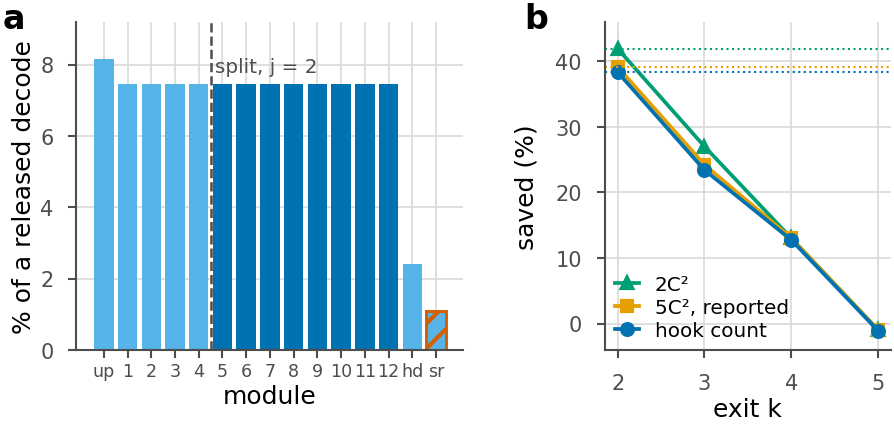
\includegraphics[width=\columnwidth]{figures/supp_b_cost.png}
\caption{\textbf{Where the arithmetic is, and what an exit saves.} \textbf{a}, one released decode by module: the opening upsample, the twelve trunk blocks, the head, and the seam-repair pass this work adds (hatched). Light bars always run; dark bars are the eight blocks after the split that a tile can skip. \textbf{b}, the saving at each reachable exit under three prices for the same architecture, with each price's ceiling dotted. Section A.5 is the table behind it.}
\end{figure}

\subsection{Every convolution in the decode}

Table 2 opens up the modules of Table 1, giving every convolution in the decode in the (K, C$_{in}$, C$_{out}$, S) convention that the architecture figures of this literature use, with the group count added because two of the shapes are depthwise. The 72 convolutions of the released decoder have only 8 distinct shapes between them, because the DepthConvBlock repeats.

\begin{table}[t]
\centering
\resizebox{\columnwidth}{!}{%
\begin{tabular}{lrrrrrrr}
\toprule
Convolution & K & C$_{in}$ & C$_{out}$ & S & Grp & MAC/px & Used \\
\midrule
up.conv.0 & 1 & 256 & 1536 & 1 & 1 & 393,216 & 1 \\
dc.0, 1$\times$1 in & 1 & 384 & 384 & 1 & 1 & 147,456 & $\times$13 \\
dc.2, 3$\times$3 depthwise & 3 & 384 & 384 & 1 & 384 & 3,456 & $\times$13 \\
dc.3, 1$\times$1 out & 1 & 384 & 384 & 1 & 1 & 147,456 & $\times$13 \\
ffn.0, 1$\times$1 C$\rightarrow$4C & 1 & 384 & 1536 & 1 & 1 & 589,824 & $\times$13 \\
ffn.2, 1$\times$1 4C$\rightarrow$C & 1 & 384 & 384 & 1 & 1 & 147,456 & $\times$13 \\
dec\_2.adaptor & 1 & 384 & 192 & 1 & 1 & 73,728 & 1 \\
head dc.0 & 1 & 192 & 192 & 1 & 1 & 36,864 & 1 \\
head dc.2, depthwise & 3 & 192 & 192 & 1 & 192 & 1,728 & 1 \\
head dc.3 & 1 & 192 & 192 & 1 & 1 & 36,864 & 1 \\
head ffn.0 & 1 & 192 & 768 & 1 & 1 & 147,456 & 1 \\
head ffn.2 & 1 & 192 & 192 & 1 & 1 & 36,864 & 1 \\
Conv1x1Adapter & 1 & 384 & 384 & 1 & 1 & 147,456 & 1 \\
FFNAdapter pw\_in & 1 & 384 & 1536 & 1 & 1 & 589,824 & $\times$4 \\
FFNAdapter pw\_out & 1 & 384 & 384 & 1 & 1 & 147,456 & $\times$4 \\
Seam repair, 3$\times$3 dw & 3 & 384 & 384 & 1 & 384 & 3,456 & 1 \\
Seam repair, 1$\times$1 & 1 & 384 & 384 & 1 & 1 & 147,456 & 1 \\
\bottomrule
\end{tabular}}
\caption{Every distinct convolution in the decode. K is the kernel side, S the stride, Grp the group count; MAC/px is per pixel of that operator's own grid, which is the latent grid for the first row and the feature grid for the rest. ``Used'' counts the instances in one decode: the DepthConvBlock appears 13 times, once in the upsample and 12 times in the trunk, and there are K $-$ 1 = 5 adapters of which four are of the FFN kind. Take from it that only two of the shapes have a kernel wider than 1$\times$1 and both are depthwise, so the 14 instances of them in one decode carry 0.34\% of the arithmetic between them.}
\end{table}

{\small results/mac\_audit.json for the released rows, results/adapter\_cost.json for ours. The two depthwise convolutions are the whole of the decoder's spatial footprint, which is why a tile boundary is cheap to repair.}

That last figure is the premise of the whole method, so it is worth stating separately: 99.66\% of the released decoder's arithmetic is 1$\times$1 convolution, which has no neighbours to miss. The receptive field of the trunk plus head grows by exactly one feature pixel per block, from 1 feature pixel with no trunk blocks to 13 with all 12, which is 104 RGB px per tile edge (results/dmc\_ld\_rf\_probe.json, measured on the released DCVC checkpoints rather than ours). A tile decoded alone is therefore wrong only in a band, and the band is narrower for a tile that exits early.

The two DepthConvBlock widths obey the same closed form. Writing the block as a 1$\times$1 projection, a 3$\times$3 depthwise, a second 1$\times$1 and a feed-forward pair whose first 1$\times$1 expands to 4C and whose gated activation folds 4C back to C for free, the closing 1$\times$1 is C$\rightarrow$C rather than 4C$\rightarrow$C and the block is

\begin{equation}
M_{\mathrm{block}}(C) = C^2 + 9C + C^2 + 4C^2 + C^2 = 7C^2 + 9C,
\end{equation}

which is 1,035,648 MAC/px at C = 384 and 259,776 at C = 192, both matching Table 2 row by row. The arithmetic model in flexuf/cost.py, which runs inside the allocation's argmin and nowhere else, writes the block as 8C$^2$ + 9C = 1,183,104 instead, so it prices a block 14.24\% high. Section A.6 measures what that is worth against a hook count.

\subsection{What the ladder adds}

Three modules are new. An exit that stops early hands the head a feature map the remaining blocks would have refined, and an \emph{adapter} stands in for them. The 1$\times$1 adapter is f + Wf with W a C$\times$C matrix. The FFN adapter repeats the block's feed-forward pair, a 1$\times$1 expanding C$\rightarrow$4C, the same gated activation, and a 1$\times$1 C$\rightarrow$C. Both are zero-initialised, so the ladder is the released decoder exactly at step zero and any quality the adapters add is attributable to them. Neither has a spatial footprint, so neither widens the seam. The \emph{seam repair} is a gated depthwise 3$\times$3 followed by a zero-initialised 1$\times$1, run once on the stitched canvas after unpatchify and before the head, which is the only place a 3$\times$3 can see across a tile boundary. The \emph{router head} reads the shared stem and predicts a per-tile exit; Section F is its architecture and this section only prices it.

\begin{table}[t]
\centering
\resizebox{\columnwidth}{!}{%
\begin{tabular}{lrrrrr}
\toprule
Module & Operators & MAC/px & In C$^2$ & Blocks & Of decode \\
\midrule
1$\times$1 adapter & 1$\times$1 C$\rightarrow$C & 147,456 & 1.00 & 0.1424 & 1.061\% \\
FFN adapter & 1$\times$1 C$\rightarrow$4C, 1$\times$1 C$\rightarrow$C & 737,280 & 5.00 & 0.7119 & 5.306\% \\
Seam repair & 3$\times$3 dw, 1$\times$1 C$\rightarrow$C & 150,912 & 1.02 & 0.1457 & 1.086\% \\
Router head & two 1$\times$1, then an MLP & n/a & n/a & n/a & \RouterCostPct\% \\
\bottomrule
\end{tabular}}
\caption{What the ladder adds, priced against one released decode. ``Blocks'' is the module in units of a trunk block. Take from it that the FFN adapter costs 5C$^2$ per pixel: the gated activation is free, so the pair is 4C$^2$ + C$^2$ rather than 4C$^2$ + 4C$^2$, and the module is 0.71 of a whole block. The routed allocation lives at exits 2 and 3, which both wear it, so it is priced where the reported saving leans hardest.}
\end{table}

{\small results/adapter\_cost.json for the two adapters, on the pinned checkpoint. The seam-repair row is 9C + C$^2$ per pixel; Section A.6 confirms that figure against a hook count rather than taking it from the source. Router: results/router\_latency.json.}

The ladder assigns the FFN adapter to any exit skipping four or more blocks and the 1$\times$1 adapter otherwise, which at K = 6 and b = 2 means the FFN at exits 0 to 3, the 1$\times$1 at exit 4, and no adapter at exit 5, whose feature is the trunk's own output with nothing standing in for a skipped block. The arithmetic at exit 5 is therefore the released decoder's, plus the repair pass, which is why the deepest exit costs slightly more than the release rather than the same.

\subsection{From the block to the decoder}

Write s$_{up}$, s$_{trunk}$ and s$_{head}$ for the shares of a released decode taken by the upsample, the trunk and the head; a$_{k}$ for the adapter at exit k; and r for the seam-repair pass. A tile assigned an exit shallower than j still runs group j, because the decoder clamps the map, so the cost of exit k in units of one released decode is

\begin{equation}
c_k = s_{\mathrm{up}} + s_{\mathrm{head}} + r + s_{\mathrm{trunk}}\frac{(\max(k,j)+1)b}{N} + a_{\max(k,j)},
\end{equation}

and the frame-level cost of an exit map a over T tiles amortises the shared part over the frame rather than over the tile,

\begin{equation}
C(a) = s_{\mathrm{up}} + s_{\mathrm{trunk}}\frac{jb}{N} + s_{\mathrm{head}} + r + \frac{1}{T}\sum_{i=1}^{T} u_{a(i)},
\end{equation}

with u$_{k}$ the per-tile suffix, meaning the blocks after the split plus the adapter. Only the last term depends on the map. That is the structural reason a ladder over a decoder of this shape has a ceiling well below 100\%: at the split depth the upsample, the first jb = 4 blocks, the head and the repair pass are already 41.5\% of a released decode, and they run whatever the map says.

None of the four shares has to be taken on trust. results/mac\_audit.json gives s$_{up}$ = 0.0816, s$_{trunk}$ = 0.8944 and s$_{head}$ = 0.0240 by hook count, so one trunk block is 0.074533 of a decode. That figure has an independent check. results/static\_RECIPE512\_b01.json records the frame-level saving of a map that sends every tile to exit e, for e = 2 to 5, on the pinned checkpoint; differencing consecutive entries gives one trunk block as 0.074533, which agrees with the audit to 7$\times$10$^{-7}$ of a decode. One is a shape audit of the released decoder with no weights loaded and the other is a set of measured savings on ours, which is the reason to report both.

\subsection{The per-exit cost vector and the ceiling}

\begin{table}[t]
\centering
\resizebox{\columnwidth}{!}{%
\begin{tabular}{lrrrrr}
\toprule
Exit k & Blocks & Adapter & c model & c hook & Saved \% \\
\midrule
0 (clamped) & 6 & FFN & 0.6088 & 0.6167 & 38.33 \\
1 (clamped) & 6 & FFN & 0.6088 & 0.6167 & 38.33 \\
2 & 6 & FFN & 0.6088 & 0.6167 & 38.33 \\
3 & 8 & FFN & 0.7578 & 0.7658 & 23.42 \\
4 & 10 & 1$\times$1 & 0.8697 & 0.8724 & 12.76 \\
5 & 12 & none & 1.0095 & 1.0109 & -1.09 \\
\bottomrule
\end{tabular}}
\caption{The per-exit cost vector, in units of one released decode, priced two ways: the arithmetic model the allocation's argmin runs on, and the hook count assembled in Section A.4, which is what every saving in the paper is quoted from. The two differ by most at the shallowest reachable exit, which wears the FFN adapter, and by least at exits 4 and 5, which wear the cheap adapter or none. The deepest exit costs 1.09\% \emph{more} than the release, which is the seam-repair pass.}
\end{table}

{\small Exits 0 and 1 are unreachable: the decoder clamps the map at j = 2, so a tile nominally assigned them leaves through exit 2 and wears exit 2's cost. The model vector is recorded in results/why\_qp\_PAPER.json; a cost vector is a property of the model rather than of the weights.}

The ceiling is 100(1 $-$ c$_{j}$), the saving when every tile takes the shallowest reachable exit. It is a property of the architecture and no allocation can pass it. The model reads \CeilingModelled\% and the meter 38.33\%, which is the value the paper's tables use, and the next subsection is the demonstration.

\begin{figure}[t]
\centering
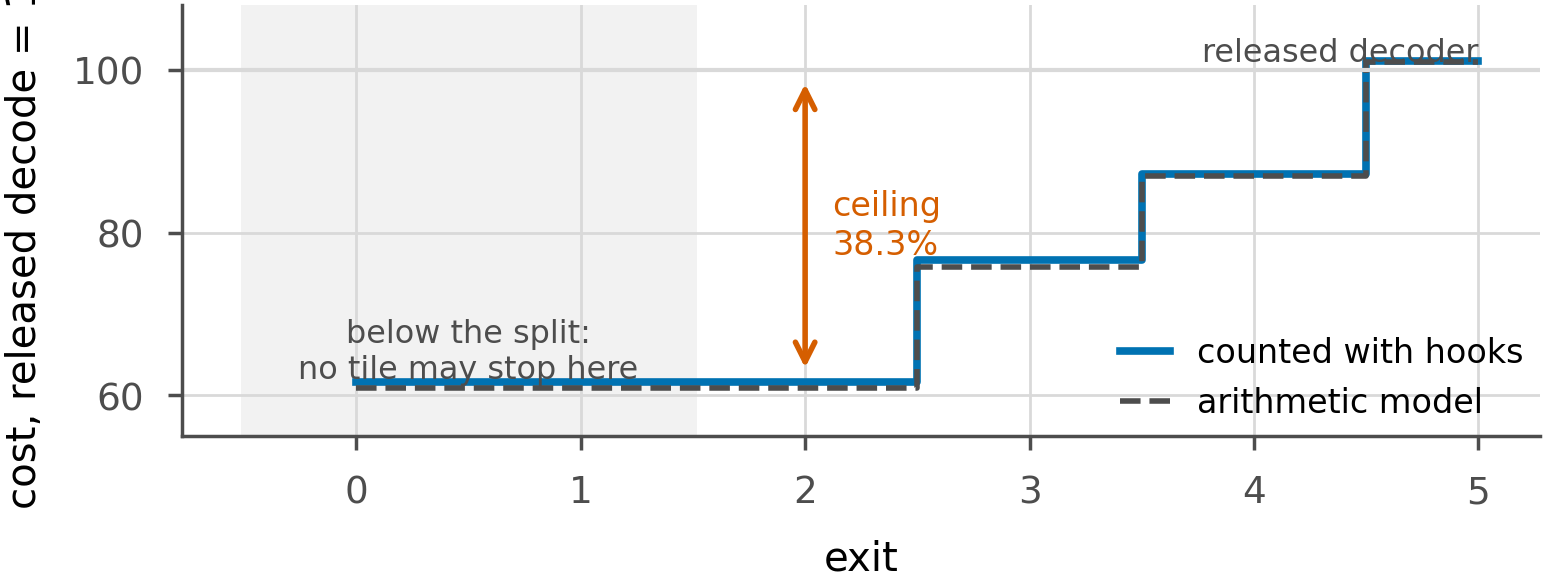
\includegraphics[width=\columnwidth]{figures/ladder.png}
\caption{\textbf{The ladder, priced.} What a tile costs at each exit, as a percentage of one released decode, counted with hooks on the executed pass and beside the arithmetic model the argmin uses. Exits below the split depth are not distinct, because the first j groups run for every tile whatever it does. The deepest exit costs slightly more than the release, which is the full-frame deblocking pass. Reported savings in the paper are the hook count.}
\end{figure}

\subsection{Predicted against hook-measured}

A cost model and the decoder it models drift apart. The check that catches it is a hook count: flexuf/measure.py attaches a forward hook to every convolution and linear layer and accumulates MACs from the output shape of each call. A group skipped by an early exit never fires its hook and so costs nothing; a group run on 28 of 40 tiles costs 28 tiles' worth, because tiles are the batch dimension and the output shape carries them. There is no bookkeeping to get wrong, and the count is the ground truth the model is judged against.

\begin{table}[t]
\centering
\resizebox{\columnwidth}{!}{%
\begin{tabular}{lrrrrrr}
\toprule
Condition & Map 2/3/4/5 & Measured & 5C$^2$ & diff & Hook & diff \\
\midrule
720p q0 & 11/4/0/0 & 34.3524 & 35.1494 & +0.797 & 34.3524 & +0.0000 \\
720p q32 & 6/4/2/3 & 23.0606 & 23.6547 & +0.594 & 23.0606 & +0.0000 \\
720p q63 & 4/3/4/4 & 18.0177 & 18.4971 & +0.479 & 18.0177 & +0.0000 \\
1080p q0 & 28/10/1/1 & 32.9763 & 33.7436 & +0.767 & 32.9763 & +0.0000 \\
1080p q32 & 16/10/6/8 & 22.8829 & 23.4682 & +0.585 & 22.8829 & +0.0000 \\
1080p q63 & 11/7/11/11 & 17.8489 & 18.3184 & +0.470 & 17.8489 & +0.0000 \\
\bottomrule
\end{tabular}}
\caption{Predicted against measured, on six decodes with six different exit maps at two resolutions. ``Measured'' is the hook count off the decode that was executed and timed. Take from it that the assembly of Section A.4 reproduces the count exactly in every condition, to four decimal places and in fact to floating point, while the model the paper reports is optimistic by 0.47 to 0.80 points and always in the same direction.}
\end{table}

{\small results/supp\_power.json, pinned checkpoint, 0.1 dB budget, NVIDIA RTX A6000. The map is the file's pooled exit histogram rounded to the frame's tile count, which is what scripts/power\_profile.py decodes; its four columns are the tiles leaving at exits 2, 3, 4 and 5.}

Because a hook count is exactly linear in the exit map, six mixtures spanning four reachable exits over-determine the per-exit vector and it can simply be solved for. The six equations are consistent to 3$\times$10$^{-16}$, and the solution differs from the assembled vector by at most 2$\times$10$^{-15}$ at any exit. The identity is worth stating plainly: the per-module counts of results/mac\_audit.json and results/adapter\_cost.json are not a model of what the meter reports, they are what the meter reports, rearranged. The residual against the model is therefore not noise and not a tolerance but a closed form: three modules are priced as a fraction of a block, the model's block is 8C$^2$ + 9C where the meter's is 7C$^2$ + 9C, and the mispricing is largest at the exits wearing the FFN adapter, which are exactly the exits the saving leans on. It comes to 0.7970 points of saving at exits 2 and 3 and 0.1354 at the deepest.

\begin{figure}[t]
\centering
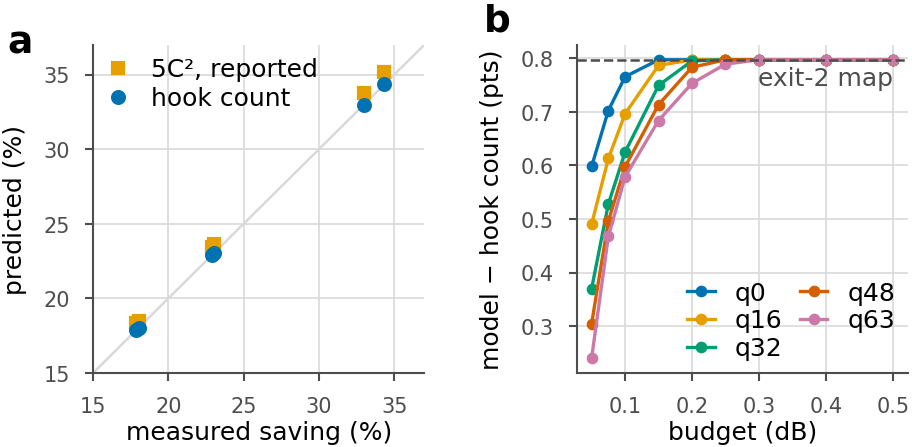
\includegraphics[width=\columnwidth]{figures/supp_b_check.png}
\caption{\textbf{The model against the meter.} \textbf{a}, six decodes at two resolutions: the hook-count assembly lies on the identity line and the model the paper reports lies above it. \textbf{b}, the same residual over the whole budget grid, 9 budgets by 5 quality indices on \NumSeq sequences. It is positive everywhere, grows with the budget, and saturates at the value an all-exit-2 map implies.}
\end{figure}

Figure 3b runs the same comparison over the whole operating range rather than six points of it. The residual is positive in all 42 cells, from 0.296 to 0.797 points, and it saturates at exactly that exits-2 value. The paper's headline figures are the hook counts, so no subtraction is left for a reader to do; had the model been quoted instead, every figure would have been between 0.43 and 0.69 points higher. At the 0.1 dB budget the model reads 29.90\% at the lowest rate where the meter reads \MainLowRate\%, and 15.64\% at the highest where the meter reads \MainHighRate\%.

{\small results/signalled\_RECIPE512\_grid.json and results/signalled\_RECIPE512\_ctc53.json, both on the pinned checkpoint. Both columns are in the files: saving\_pct\_vs\_release is the model, saving\_pct\_measured is the hook count, and model\_minus\_measured is their difference.}

\begin{table}[t]
\centering
\resizebox{\columnwidth}{!}{\begin{tabular}{lrrr}
\toprule
Decoder & GMAC & \% of release & ms \\
\midrule
Released DCVC-UF & 454 & 100.0 & 274 \\
FLEX-UF, all tiles deepest & 458 & 101.0 & 297 \\
FLEX-UF, 0.1\,dB budget & 346 & 76.2 & 196 \\
FLEX-UF, architectural ceiling & 263 & 58.1 & -- \\
\bottomrule
\end{tabular}
}
\caption{\textbf{Decoder complexity at 1080p}, in the three units a reader is likely to want: arithmetic, arithmetic as a fraction of the release, and milliseconds. Our deepest exit costs slightly more than the released decoder because it still pays the deblocking filter, and that 1.0095, not 1.0, is what every saving in the paper is \emph{not} divided by. Wall-clock is the sorted per-tile loop.}
\end{table}

{\small results/signalled\_RECIPE512\_ctc53.json and results/latency\_RECIPE512\_sorted.json, generated into paper/tables/complexity.tex by scripts/make\_paper\_tables.py. The architectural-ceiling row has no wall clock because no allocation on this test set reaches it at the budgets measured here.}

\subsection{How the timings were taken}

The rest of this section leaves arithmetic for the clock, so the protocol comes first. Everything below follows the same rules and they are stated rather than implied. Every timing, power and memory figure in this section is at the 0.1 dB budget, and every GPU figure is an NVIDIA RTX A6000, all eight cards in this machine being that model; the CPU rows are the only second device class this work can report.

\begin{itemize}\itemsep1pt
\item \textbf{Batch 1, and why.} Every wall clock here is one frame at a time, which is what a decoder does. A batch is genuinely different work for this decoder and not a repetition, because exit\_map is indexed over the whole batch's tiles, so B frames of 40 tiles form one shrinking active set of 40B and the groups run wider. Section A.8 measures what the choice costs.
\item \textbf{Warm-up, then interleaving, then the median.} 20 untimed iterations, then 40 rounds of one call of each variant in turn. This is a shared card, and timing all of the released decoder and then all of ours puts any drift in a neighbouring job's load straight into the ratio, which is the only quantity these runs exist to produce.
\item \textbf{What the timer wraps.} time.perf\_counter around a synchronised call, not CUDA events, because events do not exist on the CPU and the two device classes have to be timed alike. The timer starts at the decoded latent and stops at the reconstruction, so it includes patchify, every group, unpatchify, the seam-repair pass and the head.
\item \textbf{What is deliberately outside it.} Entropy decoding, because the bitstream and therefore the rate do not depend on the exit map: including it would divide both sides of every ratio by the same constant and flatter the method. The map itself is charged, in bits rather than in time, at \MapBits bits per frame.
\item \textbf{The router is charged in MACs and not in seconds.} Its arithmetic is \RouterCostPct\% of a decode but \RouterTimePct\% of decode time, \RouterTimeFactor$\times$ its arithmetic share, an extra \RouterTimeExtra points bought by launching a small kernel over a large map. That is the general reason a MAC count cannot see a kernel launch, in miniature (results/router\_latency.json, 40 iterations at 2048$\times$1280 on an NVIDIA RTX A6000, measured on runs/RECIPE512/ckpt\_eval.pth.tar). The router does not run at all in the signalled configuration, where the encoder chooses the map.
\item \textbf{The masked path, not the sorted one.} The shipped configuration leaves sorted\_tiles off, so every group is a masked gather over the full tile batch. Sorting the tiles by depth turns each group into a contiguous slice and recovers \WallSortedGain points at 1080p for bit-identical output (results/latency\_RECIPE512\_sorted.json, on runs/RECIPE512/ckpt\_eval.pth.tar). None of the timings below use it, so they are the slower of the two implementations.
\end{itemize}

\subsection{Where the seconds go, and on what device}

\begin{table}[t]
\centering
\resizebox{\columnwidth}{!}{%
\begin{tabular}{lrrrrr}
\toprule
Stage & MAC \% & 1080p tiles & 1080p ms & 720p tiles & 720p ms \\
\midrule
Stem: upsample + groups 0, 1 & 37.97 & frame & 41.39 & frame & 16.30 \\
Patchify & 0.00 &  & 0.21 &  & 0.09 \\
Group 2 (2 blocks, per tile) & 14.91 & 40 & 15.98 & 15 & 6.19 \\
Group 3 (2 blocks, per tile) & 14.91 & 28 & 11.24 & 10 & 4.16 \\
Group 4 (2 blocks, per tile) & 14.91 & 14 & 5.72 & 5 & 2.23 \\
Group 5 (2 blocks, per tile) & 14.91 & 9 & 3.79 & 3 & 1.30 \\
Unpatchify & 0.00 &  & 0.21 &  & 0.09 \\
Seam repair (full-frame) & 1.09 & frame & 2.07 & frame & 0.83 \\
Head & 2.40 & frame & 4.36 & frame & 1.72 \\
\bottomrule
\end{tabular}}
\caption{Where a routed decode goes, in arithmetic and in milliseconds. The MAC column is each stage's share of a released decode at full occupancy and sums to 101.09\%, which is the deepest exit's cost. Take from the table that patchify and unpatchify are free arithmetically and nearly free on the clock, that the repair pass is 1.09\% of the arithmetic and 2.4\% of this decode's clock, and that the head takes 5.1\% of the clock for 2.40\% of the arithmetic, being bandwidth-bound rather than arithmetic-bound.}
\end{table}

{\small results/supp\_latency\_1920x1080.json and results/supp\_latency\_1280x720.json, pinned checkpoint, q32, 0.1 dB budget, NVIDIA RTX A6000 taken under the evaluation lock so the card was not shared. Tile counts are that decode's own exit map, which leaves 28, 14 and 9 of 40 tiles alive in groups 3, 4 and 5.}

Patchify and unpatchify are reshapes and cost no arithmetic at all. They require the feature map to divide by the 32 px feature tile, which the encoder-side replicate padding guarantees: 1920$\times$1080 becomes 2048$\times$1280 and 40 tiles, 1280$\times$720 becomes 1280$\times$768 and 15 (results/tile\_definition.json).

\begin{figure}[t]
\centering
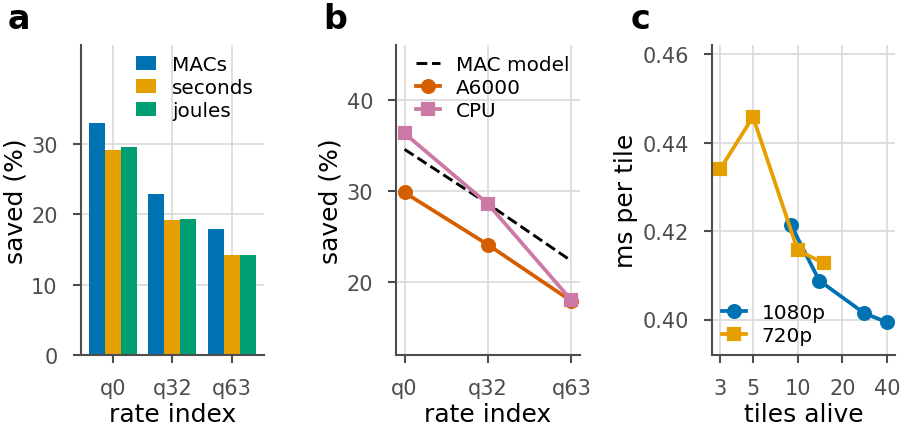
\includegraphics[width=\columnwidth]{figures/supp_b_units.png}
\caption{\textbf{What the arithmetic is worth.} \textbf{a}, one exit map measured three ways at 1080p. \textbf{b}, the same map on two device classes against what the MAC model predicts: the A6000 falls short of the prediction at every rate, the CPU does not. \textbf{c}, why a GPU falls short: a tile costs more to decode in a group that has fewer tiles left in it.}
\end{figure}

Two effects separate seconds from multiply-accumulates and the figure isolates both. The first is the tiled path itself, which the released decoder does not pay: patchify, unpatchify and the repair pass are 2.9\% of the routed clock at 1080p. Timing our own decoder with every tile at the deepest exit isolates it: that variant does the same arithmetic as the release plus the tiling machinery, and it is 2.6 to 3.8\% slower across nine measurements on the pinned checkpoint, against \TilingOverhead\% for the figure the main paper quotes. The second is occupancy. A group late in the ladder launches kernels over a handful of 32$\times$32 feature maps, and a GPU sized for the first group is partly idle inside them. Dividing each group of Table 7 by the tiles alive in it, at 1080p a tile costs 5.5\% more in group 5, on 9 tiles, than in group 2 on 40. At 720p the same curve rises by 8.0\% from 15 tiles to 5 and then falls back at 3, so the trend is clear at 1080p and not monotone at 720p.

Device class and batch size are the two knobs a reader would ask about next, and Table 8 sweeps both. All eight cards in this machine are RTX A6000s, so the only second device class reachable here is the CPU. It is also the unflattering comparison to make, in the sense that it is the one our own explanation predicts we will look better on: a CPU decode is closer to arithmetic-bound, so if the shortfall on the GPU is scheduling rather than arithmetic it should shrink.

\begin{table}[t]
\centering
\resizebox{\columnwidth}{!}{%
\begin{tabular}{lrrrrrrr}
\toprule
Device & Rate & Batch & ms/frame rel. & ms/frame ours & fps ours & Saved \% & MAC model \% \\
\midrule
A6000 & q0 & 1 & 111.3 & 78.1 & 12.8 & 29.84 & 34.58 \\
A6000 & q0 & 2 & 111.1 & 76.7 & 13.0 & 30.97 & 34.58 \\
A6000 & q0 & 4 & 110.7 & 76.5 & 13.1 & 30.96 & 34.58 \\
A6000 & q32 & 1 & 111.5 & 84.6 & 11.8 & 24.11 & 28.59 \\
A6000 & q32 & 2 & 111.3 & 83.3 & 12.0 & 25.16 & 28.59 \\
A6000 & q32 & 4 & 110.8 & 82.9 & 12.1 & 25.17 & 28.59 \\
A6000 & q63 & 1 & 111.5 & 91.5 & 10.9 & 17.92 & 22.33 \\
A6000 & q63 & 2 & 111.2 & 89.9 & 11.1 & 19.14 & 22.33 \\
A6000 & q63 & 4 & 110.7 & 89.6 & 11.2 & 19.06 & 22.33 \\
CPU, 8 thr. & q0 & 1 & 8836 & 5625 & 0.178 & 36.34 & 34.58 \\
CPU, 8 thr. & q32 & 1 & 8153 & 5822 & 0.172 & 28.59 & 28.59 \\
CPU, 8 thr. & q63 & 1 & 8280 & 6788 & 0.147 & 18.02 & 22.33 \\
\bottomrule
\end{tabular}}
\caption{Wall clock at 1080p by device class and batch size, on one exit map per rate. ``rel.'' is the released decoder timed in the same loop; fps is one over our per-frame time. Take from it that batch 1 costs about a point of saving against batch 4 and nothing beyond it, so the batch-1 convention this work uses is close to free; and that the A6000 falls short of the MAC model by 3.2 to 4.7 points at every rate and every batch size, while the CPU meets or beats it at the two lower rates.}
\end{table}

{\small results/supp\_latency\_batch\_1920x1080.json and results/supp\_latency\_cpu\_1920x1080.json, pinned checkpoint, 0.1 dB budget, exit maps read from results/supp\_paper\_curve\_PAPER.json. GPU rows: 20 warm-up and 40 interleaved iterations. CPU rows: 8 threads, 1 warm-up and 5 iterations only, on a shared machine.}

The CPU rows carry a noise floor and it should be read before the conclusion. The released decode does not depend on the rate, so its three timings should be equal; they range from 8.15 to 8.84 s, a spread of 8.4\%, which is what 5 iterations on a shared machine buys. That is enough to support the gap at q0 and q32, where the CPU is 6.5 and 4.5 points above the A6000 on the same map, and not enough to support anything at q63, where the two agree to a tenth of a point. The direction is the one the occupancy explanation predicts, and a firmer statement needs a machine that is not shared.

\subsection{What the saving is worth in joules}

Board power was sampled from the driver at 100 ms, which is about the rate the sensor updates. Each condition therefore runs for a fixed wall time of 20 s rather than a fixed iteration count, so that a 30 ms decode yields two hundred power samples rather than three. Idle is measured for 4 s immediately before and after every timed run on the same card, so a neighbouring process waking up mid-measurement appears as a drift between the two rather than as a saving. Energy per frame is the mean board power over the run times the median decode time.

\begin{table}[t]
\centering
\resizebox{\columnwidth}{!}{%
\begin{tabular}{lrrrrr}
\toprule
Condition & MACs \% & Time \% & Gap & Energy \% & Above idle \% \\
\midrule
720p q0 & 34.35 & 30.81 & 3.54 & 30.10 & 29.70 \\
720p q32 & 23.06 & 18.13 & 4.93 & 18.45 & 18.63 \\
720p q63 & 18.02 & 12.99 & 5.03 & 12.96 & 12.94 \\
1080p q0 & 32.98 & 29.07 & 3.91 & 29.56 & 29.88 \\
1080p q32 & 22.88 & 19.14 & 3.75 & 19.34 & 19.48 \\
1080p q63 & 17.85 & 14.14 & 3.71 & 14.17 & 14.18 \\
\bottomrule
\end{tabular}}
\caption{The three units side by side, all as savings of the routed decode against the released decode on the same latent. Take from it the result of this subsection: energy saved tracks time saved to within 0.5 points in every condition, while arithmetic saved runs 3.5 to 5.0 points ahead of both. Subtracting idle power changes nothing, which is the check that the agreement is not an artefact of the static draw.}
\end{table}

{\small results/supp\_power.json, pinned checkpoint, 0.1 dB budget, NVIDIA RTX A6000 with a 300 W limit, taken under the evaluation lock. 720p is padded to 1280$\times$768 and 15 tiles, 1080p to 2048$\times$1280 and 40 tiles.}

The engineering result should be stated plainly: the energy saving of this method tracks its time saving, not its arithmetic saving. A partly idle GPU still draws most of its static power, so the joules follow the seconds almost exactly, and the seconds fall short of the multiply-accumulates for the occupancy reason of Figure 4c. The routed decode draws the same board power as the released one, within 3 W in the worst of the six conditions and within 1 W in four of them, so routing does not lower the instantaneous draw of the card; it shortens the job. At 1080p and the lowest rate the three read 32.98\%, 29.07\% and 29.56\%; at the highest rate they read 17.85\%, 14.14\% and 14.17\%. Quoting the arithmetic figure as an energy figure overstates it by three and a half to five points.

Two limits. The idle baseline drifts upward as the card warms through the six conditions, so the above-idle column of Table 9 is the weaker of the two energy figures, and it is only because it agrees with the unadjusted column to within 0.4 points that the conclusion survives. Power also comes from the driver counter rather than an external meter, so the absolute joules inherit whatever bias that sensor has; the savings are ratios of two measurements taken the same way on the same card minutes apart, which is what the bias mostly cancels in.

\subsection{Memory, frame rate, and what the encoder pays}

\begin{table}[t]
\centering
\resizebox{\columnwidth}{!}{%
\begin{tabular}{lrrrrrr}
\toprule
Frame (padded) & Tiles & MB rel. & MB ours & Change \% & fps rel. & fps ours \\
\midrule
1024x512 & 8 & 180.0 & 204.0 & +13.33 & 43.89 & 49.88 \\
1280x768 & 15 & 337.5 & 382.5 & +13.33 & 22.94 & 28.03 \\
2048x1280 & 40 & 900.0 & 1020.0 & +13.33 & 9.03 & 11.18 \\
3840x2304 & 135 & out of memory &  &  &  &  \\
\bottomrule
\end{tabular}}
\caption{Peak decoder memory and frame rate, released against ours, at every resolution that fitted. Take from it that routing costs memory rather than saving it, by a constant 13.33\% at every resolution, because the tiled path holds the whole tile batch and the stitched canvas alive together; and that the frame-rate gain grows with the frame, from 43.9 to 49.9 fps at 832$\times$480 up to 9.0 to 11.2 fps at 1080p, because a larger frame has more tiles to allocate across. The 4K row is a genuine failure and is reported as one: the job ran out of memory on a 48 GB card that four other processes were sharing, so no measurement above 1080p exists anywhere in this work.}
\end{table}

{\small results/supp\_footprint.json, pinned checkpoint, q32, 0.1 dB budget, NVIDIA RTX A6000. Frame rates here are lower than in Table 8 because that table's maps are at different rates and this one is q32 throughout. Nothing above 1080p is measured anywhere in this work.}

The signalled configuration moves the choice of exit map to the encoder, which has to price the tiles before it can allocate them, and that cost is 4.52 of one tiled decode per frame per rate; section G prices the two ways of building the table and says why only one of them may be used to report quality. The asymmetry is the design rather than an accident: a decoder-side saving is bought with encoder-side work, which suits a compress-once decode-many deployment and does not suit live encoding.

{\small results/supp\_encoder\_cost\_PAPER.json: pinned checkpoint, one sequence (Bosphorus), q63, 40 tiles, 15 iterations on an NVIDIA RTX A6000.}

